\chapter{Methodology}
Folium treats an investment decision as the unit of analysis. The investor states what they intend to do with one holding, and the system answers separate questions before combining them: which pattern is most likely behind the decision (the bias model), what each choice would lead to in rupees after tax over the investor's horizon (the simulator), what generally pushes people towards this action and which habit would help (the causal module), and what the investor should do and why (the evidence rules and the explanation engine). Keeping these questions apart is the main methodological choice of the project. Each module reports only what it can support, and the recommendation rules read only the outputs they are designed to read.

The work has an offline part and an online part. Offline, the dataset is built from real market history, the bias model is trained and evaluated, and the simulator and causal module are evaluated; the outputs are model artefacts and result files. Online, for each analysis, the request and its context are captured and the five pipeline steps run. The online path only loads the offline artefacts and never retrains anything.

\section{Data Sources}
Three kinds of data are used. Daily NIFTY 50 closes and India VIX values \cite{b54} were downloaded through yfinance \cite{b52} and cached (10 June 2008 to 5 October 2026, 4,475 trading days). Monthly NIFTY 50 returns, with a 1.25\% dividend yield added, and gold returns in rupees from October 2007 to September 2026 (228 months) are cached for the simulator. Second, the synthetic investor decisions of dataset v4.1 are used for training and causal validation. Third, live share prices, mutual fund NAVs from MFAPI.in \cite{b53} and the gold price are fetched at run time and cached for 15 minutes. No real investor's trading records are used.

\section{Dataset v4.1}
There is no public dataset that links the individual decisions of Indian retail investors with their full finances and a ground-truth behavioral label, and building one would require a large consented user study. The decisions are therefore generated synthetically while the market side is kept real. The design principle is that labels are motives and not rules. Each simulated investor has hidden tendencies, the situation decides which biased motives are possible, these compete with a rational motive, and the winning motive decides both the action and the label. The same sale can therefore be rational for one investor and biased for another, and the model has to infer which from what the app can observe.

\begin{figure}[H]
\centering
\resizebox{\textwidth}{!}{\begin{tikzpicture}[node distance=4mm]
  \foreach \t [count=\i] in {{Real trading day\\ NIFTY, VIX\\ stress-\\ weighted}, {Household\\ income, EMIs,\\ rent, fees, fund}, {Portfolio\\ shares, funds,\\ gold, FD, loans}, {Hidden tendencies\\ and a possible\\ cash shock}, {Motives\\ compete\\ (bias vs rational)}, {Action and\\ label = winning\\ motive}}
    \node[box, text width=21.5mm, minimum height=19mm, font=\footnotesize, fill=\ifnum\i>4 bluefill\else tealfill\fi, draw=\ifnum\i>4 blueline\else tealline\fi] (d\i) at (\i*2.62,0) {\t};
  \foreach \i [evaluate=\i as \j using int(\i+1)] in {1,...,5} \draw[flow] (d\i) -- (d\j);
\end{tikzpicture}
}
\caption{Generation of one case in dataset v4.1}
\label{fig:datasetgen}
\end{figure}

Figure \ref{fig:datasetgen} shows the steps. A real trading day is sampled with stress over-weighted (weights of 1 for normal and bull days, 2 for corrections, 3 for euphoria and 6 for crashes) so that every motive has enough examples, and the day's real one-month return, volatility, VIX and 52-week drawdown are attached. A holding period is drawn from a log-normal distribution with a median of 14 months, and the gain or loss on the position is the real NIFTY move over that period raised to a stock beta, plus stock-specific noise. A household is then generated with age, income, years of investing, risk tolerance, horizon, rent, EMIs, education fees and an emergency fund; 14\% of borrowers carry extra debt worth 25 to 65\% of income. A portfolio of shares, funds, gold, deposits, savings, property and loans follows. Hidden tendencies are drawn, and a cash shock (job loss, medical bill or fees due) occurs with probability
\begin{equation}
P(\text{shock}) = 0.04 + 0.06\,[\text{no fund}] + 0.12\,\mathrm{clip}\!\left(\frac{0.30 - s}{0.30}, 0, 1\right),
\end{equation}
where $s$ is the surplus ratio. An emergency fund absorbs 70\% of shocks. Investors who genuinely need the money say so with probability 0.65, and others mention it with probability 0.03; this is the observable input \texttt{cash\_need\_stated}.

\begin{table}[H]
\centering
\small
\begin{tabularx}{\textwidth}{|P{2.4cm}|P{2.4cm}|P{1.6cm}|L|}
\hline
\textbf{Label} & \textbf{Motive} & \textbf{Action} & \textbf{Applies when} \\
\hline
Loss aversion & panic & sell & at a loss, NIFTY down 2\% or more over the month, and VIX $\geq$ 20 or a correction or crash \\
\hline
Loss aversion & refusal & hold & position down 25\% or more \\
\hline
Disposition effect & sell a winner & sell & up 8\% or more in a normal or rising market \\
\hline
Disposition effect & hold a loser & hold & down 5 to 25\% in a normal or rising market \\
\hline
Herd behavior & sell into fear & sell & VIX $\geq$ 22 or NIFTY down 5\% or more over the month \\
\hline
Herd behavior & buy into a rally & buy more & NIFTY up 4\% or more over the month \\
\hline
Rational & stay the course, add regularly, buy value, average down, cut a loss, rebalance, goal near, needs cash & any & the investor's own situation explains the action \\
\hline
\end{tabularx}
\caption{Label definitions used by the generator}
\label{tab:labels}
\end{table}

For a case with situation $s$ and investor $i$, the rational motive competes with weight
\begin{equation}
w_r = 0.7 + 0.025\,y_i + 0.25\,e_i + 3.0\,c_i ,
\end{equation}
where $y_i$ is years of investing, $e_i$ indicates an emergency fund and $c_i$ indicates that the money is genuinely needed. A bias motive $m$ with label $\ell$ competes with weight $w_m = S_\ell\,\tau_{i,\ell}^{1.5}\,I_m(s)$, where $\tau_{i,\ell}$ is the hidden tendency, $S_\ell$ is 3.4 for loss aversion, 2.0 for herding and 2.8 for disposition, and $I_m(s) \geq 1$ is the intensity of the situation. One motive is sampled in proportion to its weight. The large weight for a genuine cash need encodes the idea that necessity is a constraint and not a preference.

\begin{figure}[H]
\centering
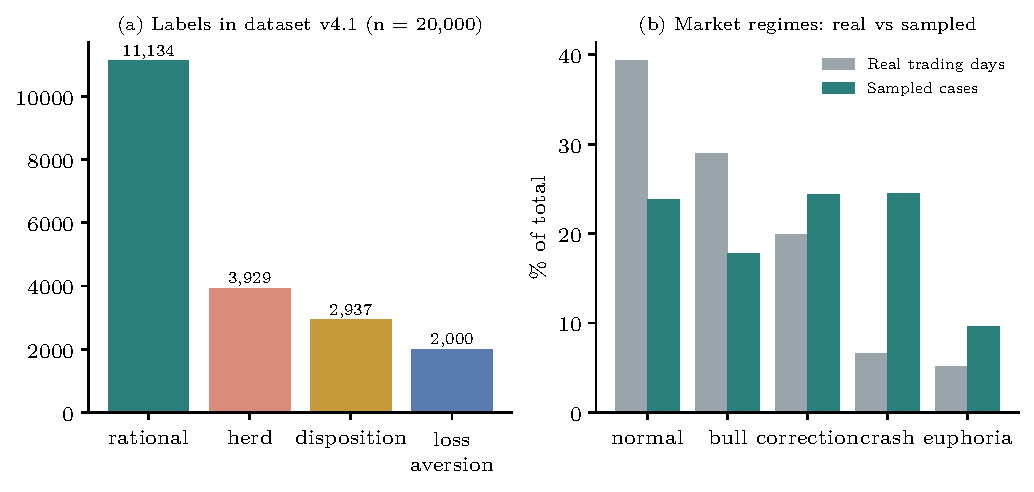
\includegraphics[width=0.95\textwidth]{figures/charts/dataset_distribution.pdf}
\caption{(a) Label distribution in dataset v4.1; (b) market regimes among real trading days and sampled cases}
\label{fig:datadist}
\end{figure}

The dataset has 20,000 cases (Figure \ref{fig:datadist}): 11,134 rational (55.7\%), 3,929 herd (19.6\%), 2,937 disposition (14.7\%) and 2,000 loss aversion (10.0\%), with 8,251 holds, 7,995 sales and 3,754 purchases. Crashes form 24.5\% of the cases against 6.6\% of real days, so every evaluation figure is re-weighted back to real regime frequencies. The median investor is 38 years old with a monthly income of \rupee 75,000 and liquid assets of \rupee 9.7 lakh, and the median position is 12\% of liquid assets. Money pressure is represented explicitly: 0.7\% of households pay out more than they earn, 44\% have no emergency fund, cash shocks hit 6.8\% of decisions, and the money is needed in 1,165 cases, 889 of which end in a forced sale.

\section{Feature Engineering}
The same function converts raw inputs into the 22 model features for training and for live requests, so the two cannot drift apart. Besides three action flags, the gain or loss, holding period, market values, age, horizon, risk tolerance and portfolio shares, two ratios are derived:
\begin{align}
\text{surplus ratio} &= \mathrm{clip}\!\left(\frac{\text{income} + \text{rent received} - \text{fixed outflow}}{\text{income}}, -2, 2\right),\\
\text{debt ratio} &= \mathrm{clip}\!\left(\frac{\text{loans}}{\text{liquid assets} + \text{property}}, 0, 5\right).
\end{align}
Three \texttt{allows} flags state which biased labels the definitions permit for this situation and action. In the product, missing profile fields are filled with training medians and missing market data with the median real trading day (NIFTY up 1.0\% in a month, VIX 16.9); all filled values are listed on the result page.

\section{Behavioral Classification}
Let $\mathbf{x} \in \mathbb{R}^{22}$ be the feature vector and $y \in \{1,\dots,K\}$ with $K = 4$. The boosted-tree score for class $k$ and its probability are
\begin{equation}
F_k(\mathbf{x}) = \sum_{m=1}^{M} f_{m,k}(\mathbf{x}), \qquad \hat{p}_k(\mathbf{x}) = \frac{e^{F_k(\mathbf{x})}}{\sum_{j=1}^{K} e^{F_j(\mathbf{x})}} ,
\end{equation}
and the training objective combines the weighted log-loss with a penalty on tree complexity \cite{b5,b26}:
\begin{equation}
\mathcal{L} = \sum_{i=1}^{n} w_i\,\ell\big(y_i, \hat{\mathbf{p}}(\mathbf{x}_i)\big) + \sum_{m,k} \Omega(f_{m,k}), \qquad \Omega(f) = \gamma T + \tfrac{1}{2}\lambda \lVert \boldsymbol{\omega} \rVert^2 ,
\end{equation}
where $T$ is the number of leaves, $\boldsymbol{\omega}$ the leaf weights and $w_i$ the ratio of the real to the sampled frequency of the case's regime.

\textbf{Guard.} Let $m_k(\mathbf{x}) = 1$ if label $k$ is allowed by the definitions, with the rational label always allowed. The guarded probabilities are $\tilde{p}_k = m_k\hat{p}_k / \sum_j m_j \hat{p}_j$, so the model can never output a pattern the definitions rule out.

\textbf{Calibration.} Let $c$ be the probability of the chosen class. A centered isotonic regression \cite{b47} fitted on out-of-fold predictions maps $c$ to a calibrated value; unlike plain isotonic regression, which is a step function, it joins the weighted centers of the constant blocks with straight lines. The calibrated value is floored so that the chosen class can never fall below the runner-up, and is capped at 0.99. Calibration is measured by the expected calibration error over ten confidence bins:
\begin{equation}
\mathrm{ECE} = \sum_{b=1}^{10} \frac{W(B_b)}{W}\,\big|\mathrm{acc}(B_b) - \mathrm{conf}(B_b)\big| .
\end{equation}
The confidence is shown to the investor as High (0.85 and above), Medium (0.65 and above) or Low.

\textbf{Attribution.} For the chosen class, SHAP decomposes the score additively, $F_k(\mathbf{x}) = \phi_{0,k} + \sum_{j} \phi_{j,k}(\mathbf{x})$ \cite{b7}, and exact TreeSHAP values \cite{b35} are summed into 18 plain drivers such as ``gain or loss'' or ``market fear''. Because Shapley values are additive this grouping is exact; the largest additivity error on the evaluation checks is $8.1\times10^{-6}$.

\section{Paired Hold versus Sell Simulation}
Let $r^E_t$ and $r^G_t$ be the monthly log-returns of NIFTY 50 and of gold in rupees. To keep the swings of history but set typical growth to stated long-run rates ($\mu_E = 11\%$, $\mu_G = 9\%$), each series is re-centered,
\begin{equation}
\tilde{r}^E_t = r^E_t - \bar{r}^E + \frac{\ln(1+\mu_E)}{12}, \qquad \tilde{r}^G_t = r^G_t - \bar{r}^G + \frac{\ln(1+\mu_G)}{12}.
\end{equation}
A path of $12H$ months is built from 12-month blocks whose starting months are drawn uniformly, with indices taken modulo the history length (a circular block bootstrap \cite{b12,b33}). The same indices are used for equity and gold, which keeps their real month-by-month relationship. Re-centering is needed because gold compounded at about 14.8\% a year from 2007 to 2026, and replaying that as the future would build an unusually strong gold boom into every path.

For a stock with beta $\beta$ and company-specific monthly volatility $\sigma$, the typical growth follows the capital asset pricing relation with the fixed deposit rate $r_f = 6.75\%$, $\mu_{\text{pos}} = r_f + \beta(\mu_E - r_f)$, and the monthly log-return on path $s$ is
\begin{equation}
\rho_{s,t} = \frac{\ln(1+\mu_{\text{pos}})}{12} + \beta\big(\tilde{r}^E_{s,t} - \bar{\tilde{r}}^E\big) + \varepsilon_{s,t}, \qquad \varepsilon_{s,t} \sim \mathcal{N}\!\left(-\tfrac{\sigma^2}{2}, \sigma^2\right).
\end{equation}
With $V_0$ the value today, $C$ the cost basis, $\kappa = 0.15\%$ the sale charges and $m_0$ the months already held, the value in hand after holding for $t$ months is
\begin{equation}
W^{(H)}_{s,t} = V_t (1-\kappa) - \mathrm{Tax}_E\big(V_t - C,\; m_0 + t\big), \qquad V_t = V_0\, e^{\sum_{u \leq t} \rho_{s,u}} .
\end{equation}
Selling realizes $P = V_0 - \mathrm{Tax}_E(V_0 - C, m_0) - \kappa V_0$ today and moves it into the investor's existing mix of gold, deposits and savings, with shares $\alpha_G, \alpha_F, \alpha_S$:
\begin{equation}
W^{(S)}_{s,t} = \alpha_G P\,G_{s,t} - \mathrm{Tax}_G(\cdot) + \alpha_F P\big(1 + r_f(1-\tau)\big)^{t/12} + \alpha_S P\big(1 + r_{sv}(1-\tau)\big)^{t/12},
\end{equation}
where $\tau$ is the investor's marginal slab rate on interest and $r_{sv} = 3\%$. Because both values are computed on the same path, their difference isolates the decision. The outputs are
\begin{align}
\tilde{\Delta}_T &= \mathrm{median}_s \big(W^{(H)}_{s,T} - W^{(S)}_{s,T}\big),\\
p &= \frac{1}{n}\sum_{s=1}^{n} \mathbf{1}\big[W^{(H)}_{s,T} > W^{(S)}_{s,T}\big],
\end{align}
together with the 10th, 50th and 90th percentiles of both paths for every year. The median is used because single-stock outcomes are right-skewed, so the mean would overstate the usual result.

\begin{table}[H]
\centering
\small
\begin{tabularx}{\textwidth}{|P{4.4cm}|L|}
\hline
\textbf{Item} & \textbf{Rule (FY 2025-26, new regime)} \\
\hline
Listed equity held 12 months or less & 20\% short-term gains tax \\
\hline
Listed equity held longer & 12.5\% on gains above \rupee 1,25,000 \\
\hline
Gold & 12.5\% after 24 months; otherwise the slab rate \\
\hline
FD and savings interest & The investor's marginal slab rate, every year \\
\hline
Cess & 4\% on top of each tax \\
\hline
Slab rate & Taxable income is gross minus \rupee 75,000; nil up to \rupee 12 lakh taxable (Section 87A rebate); above that slabs of 0, 5, 10, 15, 20, 25 and 30\% in steps of \rupee 4 lakh \\
\hline
\end{tabularx}
\caption{Tax rules used by the simulator}
\label{tab:tax}
\end{table}

The tax rules in Table \ref{tab:tax} follow the Finance (No. 2) Act, 2024 \cite{b55} and the Finance Act, 2025 \cite{b56}. The slab rate depends on income before tax, but the app records take-home pay. If $T(g)$ is the income tax on gross income $g$, including the rebate and its marginal relief, then take-home pay is $h(g) = g - T(g)$, and the simulator needs $\hat{g}$ such that $h(\hat{g})$ equals twelve times the monthly take-home pay. Since $h$ is increasing except in a short stretch of the marginal relief band, $\hat{g}$ is found by bisection with 60 iterations, and rent received is added at 70\%. For example, a take-home pay of \rupee 1.6 lakh a month corresponds to about \rupee 21.5 lakh gross, so interest is taxed at 26\% and not the 20.8\% that the take-home figure alone would give.

\section{Causal Estimation}
For a treatment $A$ and an outcome $Y$ (whether the investor takes a given action), the average treatment effect and its identification by the g-formula under consistency, positivity and conditional exchangeability given an adjustment set $Z$ are \cite{b10,b36,b37}
\begin{align}
\mathrm{ATE} &= \mathbb{E}[Y \mid \mathrm{do}(A = a')] - \mathbb{E}[Y \mid \mathrm{do}(A = a)],\\
\mathbb{E}[Y \mid \mathrm{do}(A = a)] &= \sum_{z} \mathbb{E}[Y \mid A = a, Z = z]\,P(Z = z).
\end{align}
Two estimators work from the data alone, as a real study would. G-computation fits a histogram gradient-boosting model of the action given everything observed (scikit-learn \cite{b48}, 400 iterations) and averages its predictions with the treatment set to each value. DoWhy \cite{b11} identifies the effect from a graph that mirrors the generator and estimates it with a linear model, followed by placebo, random common cause and subset refutation tests.

Because the generator is known exactly, the true effect can also be computed by re-evaluating the generator's motive probabilities with the input changed. This is what makes the evaluation possible: the estimates can be compared with the truth, which is never available in a real observational study. Gold share has no causal path to the decision and is used as a negative control. A habit is modeled as halving the tendency it acts on, which is an assumption stated in the app.

\section{Evidence-Based Recommendation}
\begin{table}[H]
\centering
\small
\begin{tabularx}{\textwidth}{|P{2.2cm}|L|}
\hline
\textbf{Intent} & \textbf{Rule} \\
\hline
Sell & $p \geq 0.60$ gives HOLD; $p \leq 0.40$ gives SELL; otherwise HOLD if the sale reads as biased, else SELL \\
\hline
Hold & $p \leq 0.40$ gives SELL; otherwise HOLD \\
\hline
Buy more & Herd behavior, or any bias with confidence $\geq 0.60$, gives HOLD; otherwise BUY MORE if $p \geq 0.50$, else HOLD \\
\hline
\end{tabularx}
\caption{Recommendation rules}
\label{tab:rules}
\end{table}

The verdict comes from the small rule set in Table \ref{tab:rules}, where $p$ is the share of simulated futures in which holding beats selling. The band between 0.40 and 0.60 is treated as a toss-up, in which the behavioral reading decides. A verdict about money should be checkable by hand, and a rule set with stated thresholds meets this need where a language model would not. Every verdict stores its reasons and the exact numbers used.

\section{Explanation}
All model outputs are gathered into one dictionary of facts. Hand-written Jinja2 \cite{b57} templates, identical in structure in English and Hindi, turn the facts into six sections: in short, what is going on right now, your two possible futures, the story of your money, why we are telling you this, and what to do now. An optional Gemini rewording is accepted only if it introduces no new number or rupee amount and its length stays between 0.6 and 1.8 times the original.

\section{Tamper-Evident Audit Chain}
Let $\mathrm{canon}(\cdot)$ be a canonical JSON serialization (sorted keys, no spaces) and $H$ be SHA-256. For the $i$-th entry of an investor, with payload $P_i$,
\begin{align}
h_0 &= H(\texttt{GENESIS:} \Vert \text{user id} \Vert \texttt{:} \Vert \text{created at}),\\
\pi_i &= H(\mathrm{canon}(P_i)), \qquad h_i = H(h_{i-1} \Vert \pi_i).
\end{align}
Changing any byte of a payload changes $\pi_i$ and therefore every later chain hash, and removing an entry leaves the next one pointing at a hash that no entry produces, following the linked time-stamping idea of Haber and Stornetta \cite{b44}. Verification walks the entries by following the links from the genesis value rather than by timestamp, and reports an entry as altered if its hashes do not recompute, as unlinked if it does not connect to the chain, and as a fork if two entries claim the same predecessor.
